\subsection{Time Course}

There are many time course analyses that
could be presented for this experiment,
and so for brevity, I report only the most informative comparisons here.
To explore the effect of varying the description
on participants' base rate-based reasoning,
I examined the proportion of trials on the side of the screen
containing the base rate-cued option,
on trials containing such an option.
Likewise, to explore the effect of varying the base rate
on description-based reasoning,
I examined the proportion of trials on the side of the screen
containing the description-cued option,
on trials such an option existed.
Both comparisons are plotted in Figure~\ref{fig:exp5_timecourse}.


\begin{figure}[ht]
  \centering
  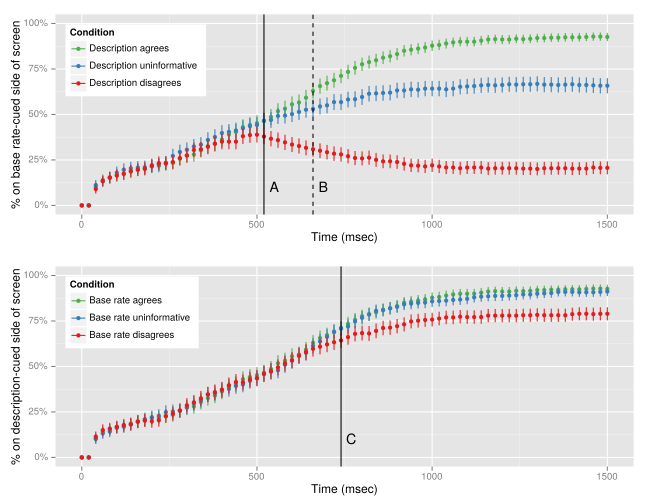
\includegraphics[width=\figurewidth]{imgs/exp5_timecourse.pdf}
  \caption[Time course plots for the effect of descriptions
    on base rate-cued choices, and vice versa, in Experiment 5.]{
    \label{fig:exp5_timecourse}
    Top: Proportion of trials where the cursor is
    on the side of the screen containing the base rate-cued option, over time,
    for trials where the description agreed with the description,
    is uninformative, or disagreed with it.
    Line A shows the onset of a significant difference between
    when the description disagreed with the base rate and the other two conditions.
    Line B shows the onset of a difference between when the description agreed
    and when it is uninformative.
    \\
    Bottom: Proportion on the side containing the description-cued option,
    for trials where the base rate agreed with the description,
    is uninformative, or disagreed with it.
    Line C shows the onset of a difference between
    when the base rate disagreed with the description and the other two conditions.
  }
\end{figure}

Divergence points were found as before,
by fitting two series of logistic mixed models.
The first predicted the proportion of trials on
the base rate-cued option's side of the screen,
with description type
(agreed with base rate, uninformative, or disagreed) as a predictor.
The second predicted the proportion of trials on
the description cued option's side of the screen,
with base rate type
(agreed with description, uninformative, or disagreed) as a predictor.
All models included random intercepts for each participant.
In each series, a model was fit to each 20 msec time window,
and divergence points for each pairwise comparison were defined as
the times after which these comparisons were found to be
statistically significant.
 
In both plots shown in Figure~\ref{fig:exp5_timecourse},
participants were equally likely to move towards each option
in any condition over the first 500 msec of each trial,
indicating that neither descriptions nor base rates
influenced participants' cursor movements before this time.

The effect of descriptions on base rate-driven reasoning was the first to manifest:
participants were significantly less likely
to place the cursor on the side of the base rate-cued option
when the description disagreed with the base rate
than when it agreed, or was uninformative,
from 520 msec onwards (line A in Figure~\ref{fig:exp5_timecourse}).
Later, they were more likely to move the cursor to this side of the screen
when the description agreed with the base rate
than when it was uninformative from 660 msec (line B in Figure~\ref{fig:exp5_timecourse}).

The effect of the base rates on description-driven reasoning was slowest to arise.
Participants became less likely to be
on the side of the screen containing the description-cued option
when the base rate disagreed with the description
than when it was agreed or was uninformative
from 740 msec onwards (line C in Figure~\ref{fig:exp5_timecourse}).
Mirroring the analysis of responses on these trials, above,
no difference emerged between
trials where the base rate agreed with the description
and trials where the base rate was uninformative.


